\documentclass[a4paper, fontsize=11pt]{scrartcl} % A4 paper and 11pt font 
\usepackage[a4paper,left=3cm,right=2cm,top=2.5cm,bottom=2.5cm]{geometry}

\usepackage[T1]{fontenc} % Use 8-bit encoding that has 256 glyphs
%\usepackage{fourier} % Use the Adobe Utopia font for the document - comment this line to return to the LaTeX default
\usepackage[spanish]{babel} % Spanish language/hyphenation
\selectlanguage{spanish}
\usepackage[utf8]{inputenc}
\usepackage{amsmath,amsfonts,amsthm} % Math packages
\usepackage{graphicx} % The graphicx package
\usepackage{placeins}
\usepackage{caption}
\usepackage{subcaption}

\usepackage{hyperref}

\usepackage{cite} % para contraer referencias


\usepackage{listings} % Insert Scripts
\usepackage{color} %red, green, blue, yellow, cyan, magenta, black, white
\definecolor{mygreen}{RGB}{28,172,0} % color values Red, Green, Blue
\definecolor{mylilas}{RGB}{170,55,241}

\lstset{language=Matlab,%
	%basicstyle=\color{red},
	breaklines=true,%
	morekeywords={matlab2tikz},
	keywordstyle=\color{blue},%
	morekeywords=[2]{1}, keywordstyle=[2]{\color{black}},
	identifierstyle=\color{black},%
	stringstyle=\color{mylilas},
	commentstyle=\color{mygreen},%
	showstringspaces=false,%without this there will be a symbol in the places where there is a space
	numbers=left,%
	numberstyle={\tiny \color{black}},% size of the numbers
	numbersep=9pt, % this defines how far the numbers are from the text
	emph=[1]{for,end,break},emphstyle=[1]\color{red}, %some words to emphasise
	%emph=[2]{word1,word2}, emphstyle=[2]{style},    
}

\usepackage{sectsty} % Allows customizing section commands
%\allsectionsfont{\centering \normalfont\scshape} % Make all sections centered, the default font and small caps

\usepackage{fancyhdr} % Custom headers and footers
\pagestyle{fancyplain} % Makes all pages in the document conform to the custom headers and footers
\fancyhead{} % No page header - if you want one, create it in the same way as the footers below
\fancyfoot[L]{} % Empty left footer
\fancyfoot[C]{} % Empty center footer
\fancyfoot[R]{\thepage} % Page numbering for right footer
\renewcommand{\headrulewidth}{0pt} % Remove header underlines
\renewcommand{\footrulewidth}{0pt} % Remove footer underlines
\setlength{\headheight}{13.6pt} % Customize the height of the header

\numberwithin{equation}{section} % Number equations within sections (i.e. 1.1, 1.2, 2.1, 2.2 instead of 1, 2, 3, 4)
\numberwithin{figure}{section} % Number figures within sections (i.e. 1.1, 1.2, 2.1, 2.2 instead of 1, 2, 3, 4)
\numberwithin{table}{section} % Number tables within sections (i.e. 1.1, 1.2, 2.1, 2.2 instead of 1, 2, 3, 4)

%\setlength\parindent{0pt} % Removes all indentation from paragraphs - comment this line for an assignment with lots of text

\newenvironment{myalign}{\par\nobreak\large\noindent\align}{\endalign} %Altering fontsize in equations globally

%----------------------------------------------------------------------------------------
%	TITLE SECTION
%----------------------------------------------------------------------------------------

\newcommand{\horrule}[1]{\rule{\linewidth}{#1}} % Create horizontal rule command with 1 argument of height

\title{	
	\normalfont \normalsize 
	\textsc{Máster en Automática y Robótica - UPM} \\ [25pt] % Your university, school and/or department name(s)
	\horrule{0.5pt} \\[0.4cm] % Thin top horizontal rule
	\huge Trabajo 1a de Cinemática de Robots \\ % The assignment title
	\horrule{2pt} \\[0.5cm] % Thick bottom horizontal rule
}

\author{Jorge Camarero Vera - 07052} % Your name

\date{\normalsize\today} % Today's date or a custom date

\begin{document}
	\maketitle
	
	\section{Explicación de la tarea}
	
	Desarrollar una función en Matlab con las siguientes especificaciones\footnote{Se ha continuado la \textbf{Parte 2} del trabajo en la misma memoria de la \textbf{Parte 1} para tenerlo todo junto.}:
	
	\begin{enumerate}
		\item Recibirá como dato los parámetros de DH de un robot de un mínimo de 2 y un máximo de 7 gdl.
		\item Permitirá definir los valores de las coordenadas articulares. Estos podrán variarse mediante sliders. En caso de grados de libertad de rotación, las unidades serán grados sexagesimales.
		\item Representará los valores de localización del extremo del robot en el espacio de la tarea pudiéndose escoger (mediante un botón de selección) entre:
		\begin{itemize}
			\item Posición del extremo en coordenadas cartesianas (XYZ) y ángulos de Euler WUW.
			\item Matriz de Transformación Homogénea del extremo.
		\end{itemize}
		\item Representará en \textquotedblleft alambres\textquotedblright al robot en las coordenadas indicadas.
		\item Se mostrará el valor numérico de la matriz Jacobiana.
		\item Si número de ejes es $>=$ número de grados de libertad se mostrará el indice de Yoshikawa en las coordenadas indicadas.
		\item Mostrará en una ventana independiente los vectores $Jv1,\,Jv2,\,Jv3,\,Jv4,\,Jv5,\,Jv6$.
		\item Mostrará en una ventana independiente los vectores $Jw1,\,Jw2,\,Jw3,\,Jw4,\,Jw5,\,Jw6$.
		\item  Representará mediante mapa de colores el valor del índice de Yoshikawa en el espacio XYZ. Para ello, se fijará el valor de uno de los ejes X, Y, Z (valor ajustable por slider) y en el dibujo de 2 dimensiones se coloreará cada punto accesible por el robot con un color variable según el rango del índice de Yoshikawa.
	\end{enumerate}
	
	%\begin{figure}[h!]
	%	\centering
	%	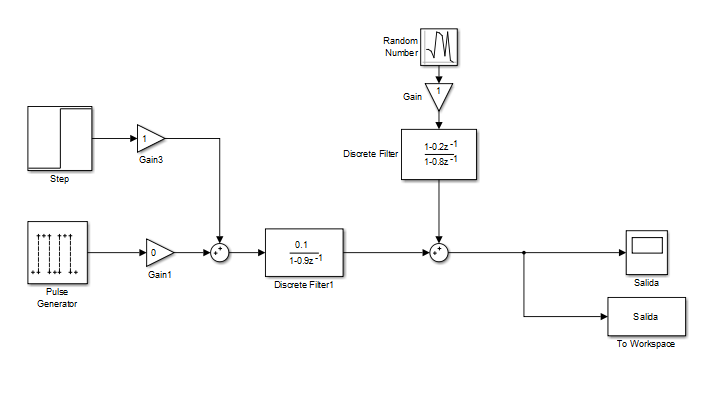
\includegraphics[width=1.0\linewidth]{images/Original_System.PNG}
	%	\caption{Modelo inicial}
	%	\label{Modelo Inicial}
	%\end{figure}
	%\FloatBarrier
	
	\section{Desarrolo del Programa - PARTE 1}
	
	Se ha creado una interfaz gráfica, GUI, para manejar las entradas y salidas que se piden para la realización de este trabajo. La GUI se ha dividido en cuatro paneles y un plot para representar el robot. Estos cuatro paneles son:
	
	\begin{itemize}
		\item Parámetros de Denavid-Hartenberg
		\item Configuraciones del Robot
		\item Rotaciones
		\item Coordenadas de la herramienta
	\end{itemize}
	
	\subsection{Parámetros de Denavid-Hartenberg} \label{Denavid-Hartenberg}
	
	En este panel, Figura \ref{Parametros}, hay una tabla para introducir los parámetros de DH, un botón para establecer los grados de libertad de la tabla anterior, una pestaña para seleccionar si se desean introducir los parámetros que implicar rotaciones en grados o en radianes, otra pestaña para establecer parámetros de DH de robots ya predefinidos. Por último se encuentra el botón de calcular que permite obtener a partir de los parámetros introducidos y las rotaciones dadas, el plot del robot y las coordenadas de las herramientas y/o su matriz homogénea.\\
	
	\begin{figure}[h!]
		\centering
		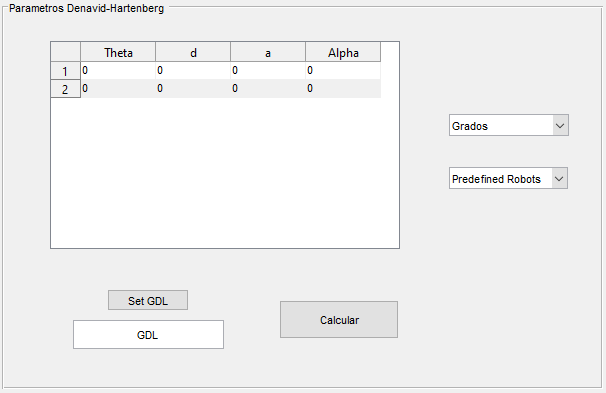
\includegraphics[width=0.8\linewidth]{images/Param.PNG}
		\caption{Panel por defecto de Parámetros de Denavid-Hartenberg}
		\label{Parametros}
	\end{figure}
	\FloatBarrier
	
	La tabla para escribir los parámetro de DH por defecto viene para 2 gdl, pero se puede cambiar abajo estableciendo los GDL que uno quiera desde 0 hasta infinito (probado hasta 1 millón), Figura \ref{Parametros_Inf}. Por lo que así conseguimos abrir el camino para representar robots sobreactuados por encima de 7 gdl.\\
	
	\begin{figure}[h!]
		\centering
		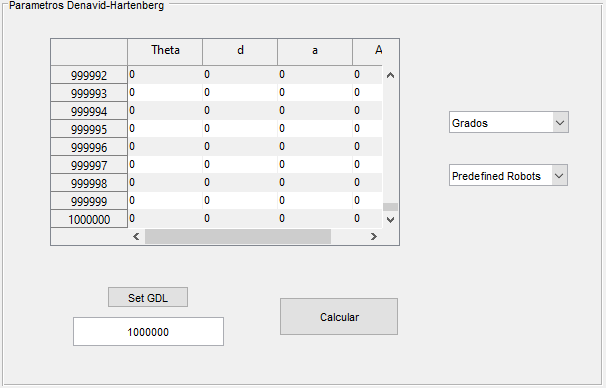
\includegraphics[width=0.8\linewidth]{images/Param_Inf.PNG}
		\caption{Panel de Parámetros de Denavid-Hartenberg con 1 millón de GDL}
		\label{Parametros_Inf}
	\end{figure}
	\FloatBarrier
	
	A la hora de ir probando la interfaz era incómodo estar cargando a mano una y otra vez los parámetros de los robots, por lo que se creó la pestaña con distintos robots predefinidos para ir probando, la lista abarca robots que se encuentran dentro de la toolbox de robótica, pero en el código los parámetros de DH los he escrito a mano, por lo que sólo han tenido que ser escritos una vez. Esto aporta ventajas de cara a la depuración del código y del uso del programa, ya que se cargan robots ya existentes, y por tanto podemos trabajar con ellos sin tener que conocer de antemano sus parámetros de DH.\\
	
	En el ejercicio se pedía para las rotaciones que los datos se introdujeran en grados sexagesimales, como desconocía si se refería también a la tabla de parámetros de DH, ha sido creada una pestaña para seleccionar si se quieren introducir los parámetros rotacionales en grados o radianes. Si se selecciona un robot predefinido habrá que establecer la pestaña en radianes, ya que estos se establecen en la tabla en radianes.\\
	
	Sobre la tabla para introducir los parámetros de DH, como se ve en la Figura \ref{Parametros}, no aparece el offset típico de la función \textit{Link} de la toolbox de robótica. Esto lo he solucionado introduciendo los parámetros de manera natural como se ha explicado en clase, Figura \ref{Parametros_DH}. Esto se consigue haciendo que la tabla reciba los parámetros como \textit{strings} y mediante expresiones regulares ir separando unas partes de otras y mover ambas partes a donde se corresponden en la función \textit{Link} de la toolbox de robótica. Vemos que también se puede escribir números como \textit{pi}.\\
	
	\begin{figure}[h!]
		\centering
		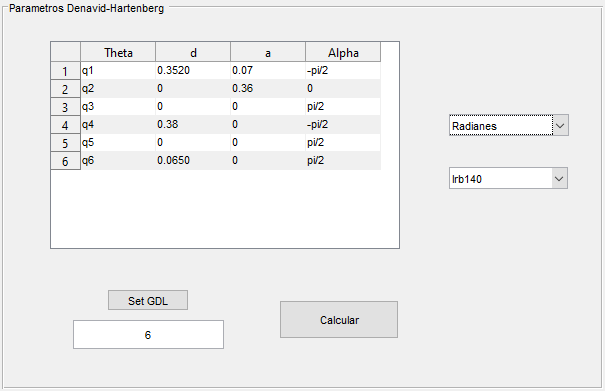
\includegraphics[width=0.8\linewidth]{images/Param_DH.PNG}
		\caption{Panel de Parámetros de Denavid-Hartenberg con datos introducidos}
		\label{Parametros_DH}
	\end{figure}
	\FloatBarrier
	
	A la hora de presionar el botón \textit{Calcular} para obtener los datos requeridos emplea los parámetros de DH que hemos dado, las rotaciones introducidas y las configuraciones del robot, estos dos últimos se explica en los siguientes apartados.\\
	
	\subsection{Rotaciones}
	
	Las rotaciones, de 1 a 7, se introducen en grados sexagesimales o bien mediante los \textit{sliders}, van de -180º a 180º, o bien mediante la tabla presente en el panel, Figura \ref{Rotaciones}. Al introducir los datos en la table automáticamente se mueven los \textit{sliders} y viceversa. Si los gdl que se introducen para el robot son inferiores al número de rotaciones introducidas el programa ignorará las rotaciones sobrantes.\\
	
	\begin{figure}[h!]
		\centering
		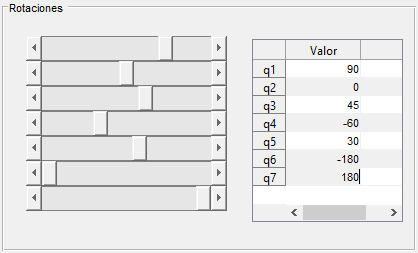
\includegraphics[width=0.6\linewidth]{images/Rotaciones.PNG}
		\caption{Panel de Rotaciones}
		\label{Rotaciones}
	\end{figure}
	\FloatBarrier
	
	\subsection{Configuraciones del Robot}
	
	En el panel de configuraciones del robot, Figura \ref{Configuraciones}, se pueden introducir matrices homogéneas de la herramienta y la base, para desplazar el origen o rotarlo, además de vector de gravedad. Aunque esto explícitamente no se pedía para este trabajo lo he introducido ya que ciertos robots predefinidos tenían modificados estos parámetros, y se decidió incluirlo en la GUI.\\
	
	\begin{figure}[h!]
		\centering
		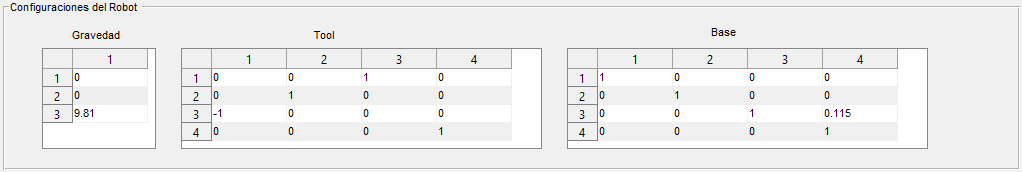
\includegraphics[width=1.0\linewidth]{images/Config.PNG}
		\caption{Panel de Configuraciones del Robot. Con los datos del robot P8 de 8 gdl y modificación extra de la posición de la base.}
		\label{Configuraciones}
	\end{figure}
	\FloatBarrier
	
	\subsection{Coordenadas de la Herramienta}
	
	En este trabajo se pide representar los valores de localización del extremo del robot en el espacio de la tarea pudiéndose escoger (mediante un botón de selección) entre:
	
	\begin{itemize}
		\item Posición del extremo en coordenadas cartesianas (XYZ) y ángulos de Euler WUW.
		\item Matriz de Transformación Homogénea del extremo.
	\end{itemize}
	
	Para completar esta tarea se ha creado una pestaña para seleccionar la salida deseada, y estos datos salen por una de las dos tablas, la de la izquierda para la posición del extremo en coordenadas cartesianas (XYZ) y ángulos de Euler WUW, y la de la derecha para la matriz de transformación homogénea del extremo, Figura \ref{Output}.\\
	
	\begin{figure}[h!]
		\centering
		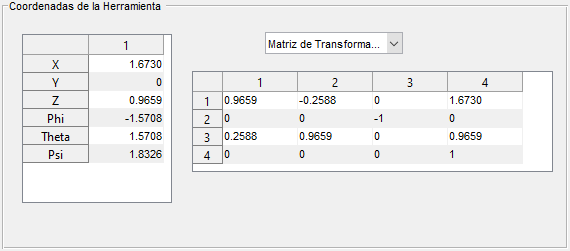
\includegraphics[width=0.8\linewidth]{images/Output.PNG}
		\caption{Panel de Coordenadas de la Herramienta.}
		\label{Output}
	\end{figure}
	\FloatBarrier
	
	Estos resultados se obtienen automáticamente al pulsar el botón \textbf{Calcular} en el panel de parámetros Denavid-Hartenberg. Si primero se selecciona las coordenadas y se pulsa calcular, y después se selecciona la matriz de transformación homogénea y se vuelve a calcular se mantienen los resultados en ambas tablas.\\
	
	\subsection{Plot del Robot}
	
	Al pulsar el botón \textbf{Calcular} también se genera un plot en tres dimensiones en el que se muestra el robot en la posición calculada, Figura \ref{Plot}.
	
	\begin{figure}[h!]
		\centering
		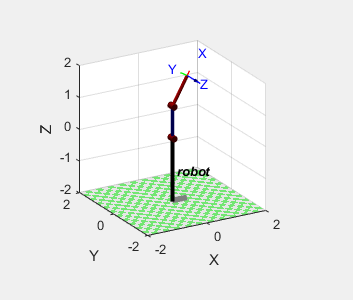
\includegraphics[width=0.6\linewidth]{images/Plot.PNG}
		\caption{Plot en 3D de la posición calculada de un robot con 2 gdl.}
		\label{Plot}
	\end{figure}
	\FloatBarrier
	
	\section{Pruebas hechas con distintos robots y grados de libertad}
	
	Se han hecho pruebas para el correcto funcionamiento de la GUI que van desde robots de 1 gdl, Figura \ref{GDL1}, hasta 8 gdl, Figuras \ref{GDL8} y \ref{GDL8_J}, éste último presenta GDL tanto rotacionales como prismáticos. Pese a que los parámetros de DH se introducen en radiantes para introducir las rotaciones se deberán hacer en grados sexagesimales, Figura \ref{GDL3}.
	
	\begin{figure}[h!]
		\centering
		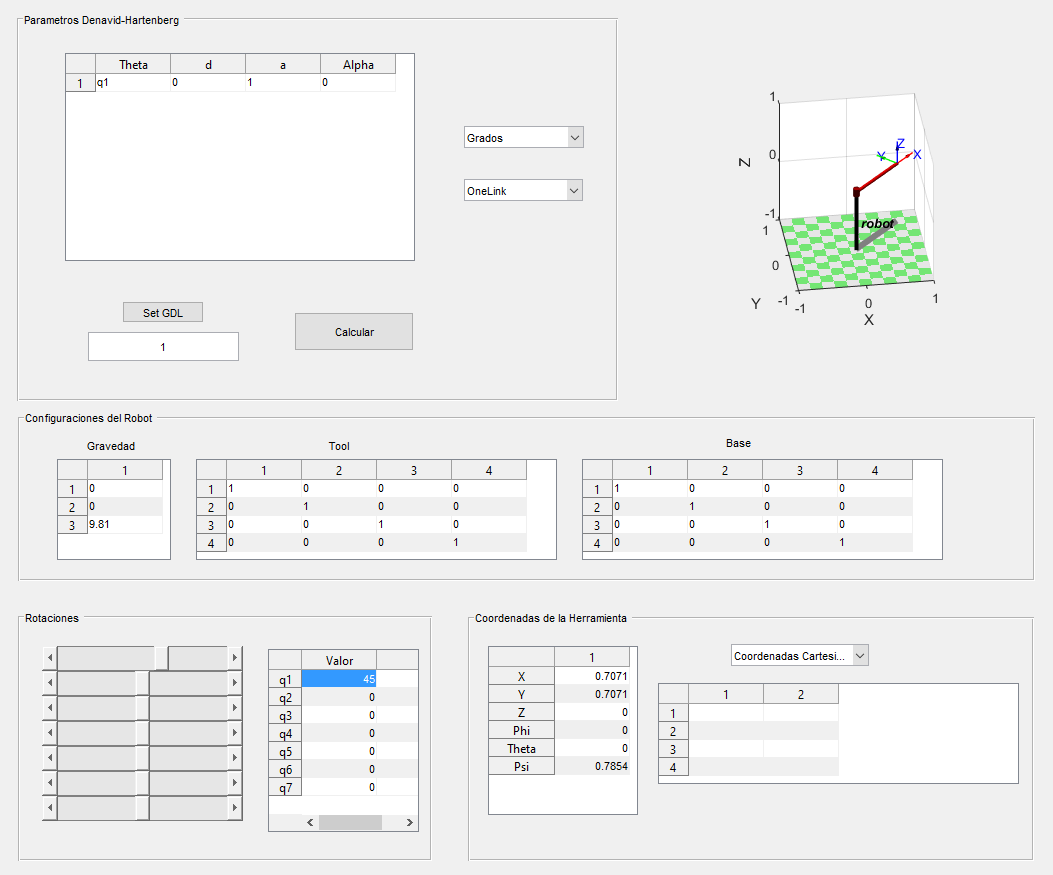
\includegraphics[width=1.0\linewidth]{images/GDL1.PNG}
		\caption{GUI presentando los datos de un robot con 1 gdl.}
		\label{GDL1}
	\end{figure}
	\FloatBarrier
	
	\begin{figure}[h!]
		\centering
		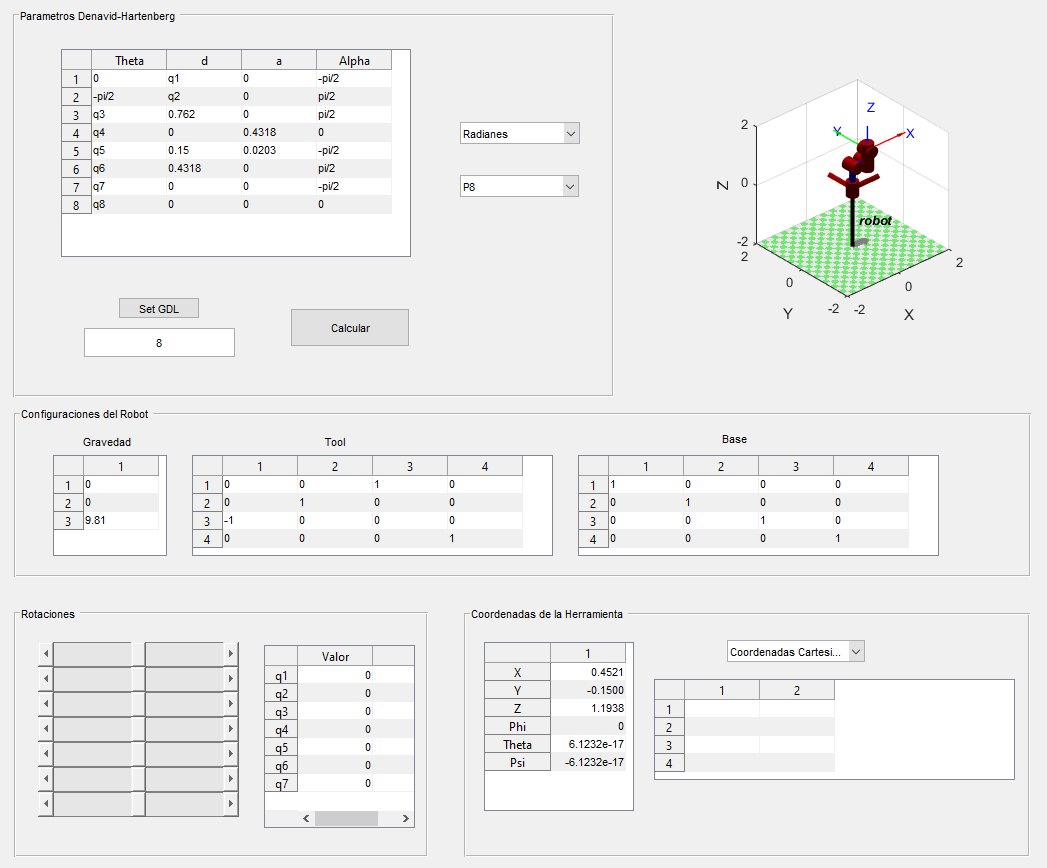
\includegraphics[width=1.0\linewidth]{images/GDL8.PNG}
		\caption{GUI presentando los datos de un robot con 8 gdl, es el robot predefinido \textit{P8}.}
		\label{GDL8}
	\end{figure}
	\FloatBarrier
	
	\begin{figure}[h!]
		\centering
		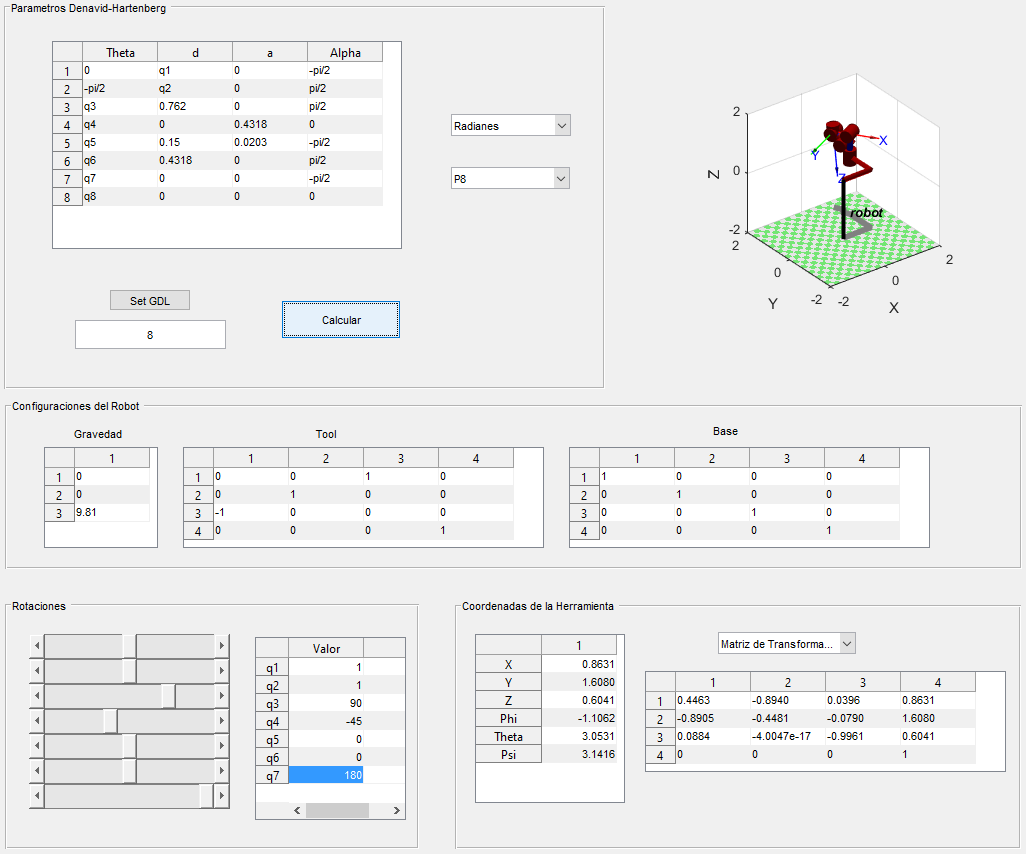
\includegraphics[width=1.0\linewidth]{images/GDL8_J.PNG}
		\caption{GUI presentando los datos de un robot con 8 gdl, es el robot predefinido \textit{P8}. Se han establecido rotaciones y movimientos en gdl prismáticos.}
		\label{GDL8_J}
	\end{figure}
	\FloatBarrier
	
	\begin{figure}[h!]
		\centering
		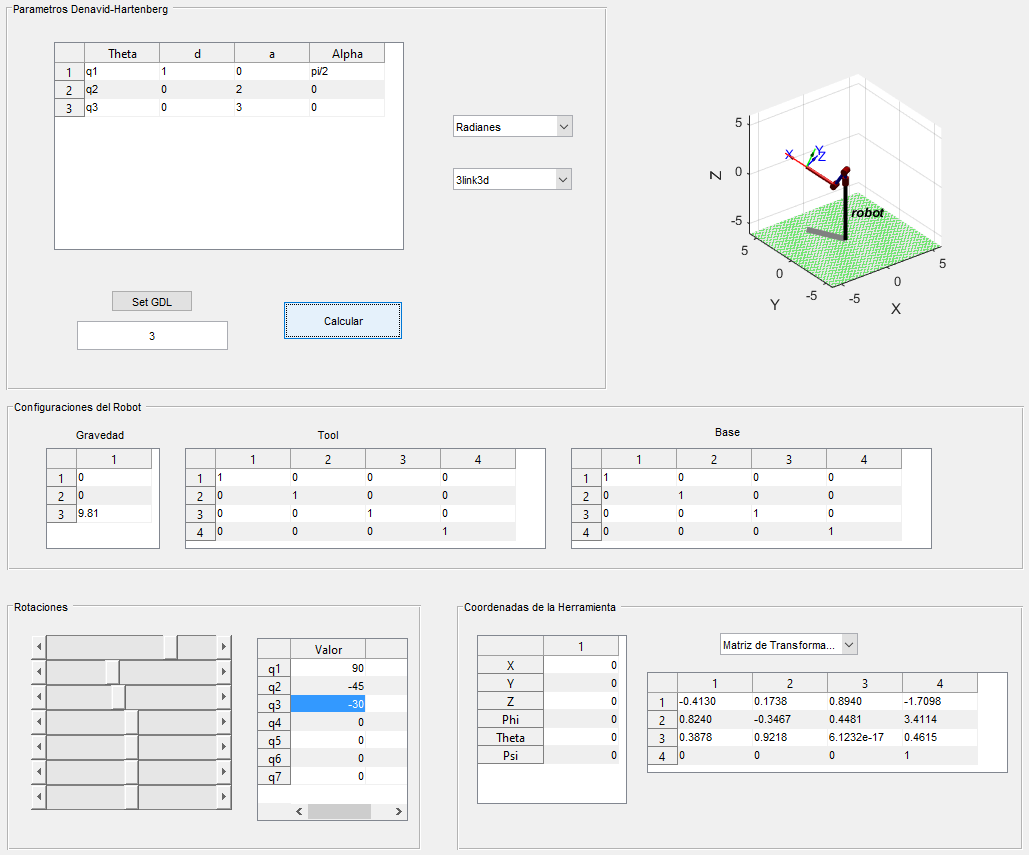
\includegraphics[width=1.0\linewidth]{images/GDL3.PNG}
		\caption{GUI presentando los datos de un robot con 3 gdl. Las rotaciones son en grados sexagesimales y se pide calcular la matriz de transformación homogénea.}
		\label{GDL3}
	\end{figure}
	\FloatBarrier
	
	\section{Desarrollo del Programa - PARTE 2}
	
	Se ha continuado ampliando el programa y la GUI desarrollado en la \textbf{Parte 1} conforme a las peticiones de la \textbf{Parte 2} del \textit{Trabajo 1} pedido para la presente asignatura.\\
	
	La GUI ha sido ampliada con 2 paneles nuevos:
	
	\begin{description}
		\item[Yoshikawa] Figura \ref{Yoshi_Panel}. En este panel aparecen el indice de Yoshikawa calculado para las coordenadas articuladas precisadas. Además de poder mostrar el valor del índice de Yoshikawa en el espacio XYZ. 
		\item[Jacobian] Figura \ref{Jacobian_Panel}. En este panel se representa la Jacobiana calculada para las coordenadas articuladas precisadas. Y además la representación de sus vectores.
	\end{description}
	
	\begin{figure}[h!]
		\centering
		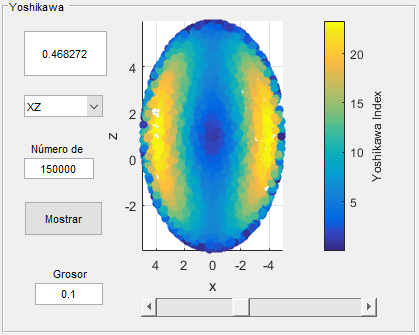
\includegraphics[width=0.6\linewidth]{images/YoshiPanel.PNG}
		\caption{Panel de Yoshikawa}
		\label{Yoshi_Panel}
	\end{figure}
	\FloatBarrier
	
	\begin{figure}[h!]
		\centering
		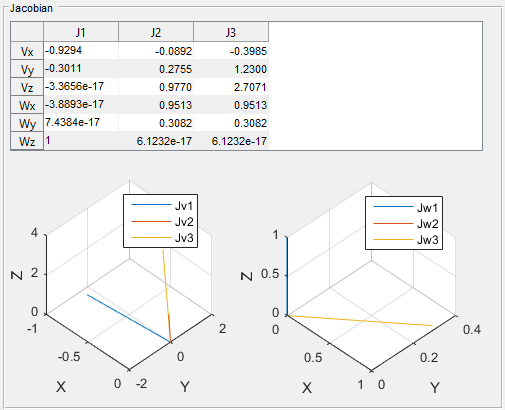
\includegraphics[width=0.6\linewidth]{images/JacobianPanel.PNG}
		\caption{Panel de la Jacobiana}
		\label{Jacobian_Panel}
	\end{figure}
	\FloatBarrier
	
	\subsection{Yoshikawa}
	
	En determinadas zonas del área de trabajo, el robot puede moverse bien en todas las direcciones (Jacobiana bien condicionada Coliumnas de J linealmente independientes). En otras zonas, en determinadas direcciones no tiene facilidad de movimiento (Jacobiana mal condicionada). El índice de maniobrabilidad da una medida escalar de esta dificultad de movimiento. El índice de Yoshikawa es:
	
	\begin{myalign}
		\eta = \sqrt{det(J(q))\cdot J^T(q)}
	\end{myalign}
	%
	Si J tiene más filas que columnas el índice vale siempre 0 (el robot tiene menos \textit{gdl} que los necesarios por lo que su maniobrabilidad o capacidad para moverse en cualquier dirección del espacio de la tarea es nula). Se acerca a $0$ para zonas de difícil movimiento y es grande en zonas de movimiento posible en todas las direcciones.\\
	
	El cálculo del índice de Yoshikawa para las coordenadas articulares dadas se realiza cuando se pulsa el botón \textit{Calcular} de la sección \ref{Denavid-Hartenberg}. Este cálculo se hace de la siguiente manera:
	
	\begin{lstlisting}
	% qs , vector coordenadas articulares
	yoshikawa = robot.maniplty(qs, 'yoshikawa');
	\end{lstlisting}
	%
	Previamente se han tenido que definir las coordenadas articulares que se desean para el cálculo del \textit{índice de manipulabilidad de Yoshikawa}. Este índice aparece en la GUI en el cuadro superior del panel de Yoshikawa.\\
	
	Para mostrar los índices de manipulabilidad de Yoshikawa en todo el espacio de tareas ha sido una labor de gran capacidad de cómputo, ya que habría que asignar el número suficiente de puntos del espacio en todo el volumen de la tarea, probando distintos conjuntos de puntos se ha conseguido ver un óptimo con $150.000$ puntos, aunque esto puede variar de un robot a otro. Por esta razón se ha implementado en el panel un cuadro para especificar el número de puntos deseado (por defecto $150.000$).\\
	
	El cálculo se realiza mediante la función \textit{Yoshikawa\_W(hObject, handles, robot)}, se ha seguido el siguiente esquema:
	
	\begin{enumerate}
		\item Generar puntos cuasi-aleatorios en el espacio articular. Esto se ha conseguido mediante la función \textit{sobolset}\footnote{La clase \textit{sobolset} construye un conjunto de puntos cuasi-aleatorios de Sobol. $p = sobolset(d)$ construye un $d$-dimensional conjunto de puntos $p$ de la clase \textit{sobolset}, con las configuraciones de propiedades por defecto. \href{http://es.mathworks.com/help/stats/sobolset.html}{sobolset}.}.
		
		\item Extraer los primeros $N$ puntos del conjunto de \textit{Sobol}. Para esto se ha empleado la función \textit{net}\footnote{$X = net(p,n)$ devuelve los primeros $n$ puntos en $X$. \href{http://es.mathworks.com/help/stats/qrandset.net.html}{net}.}
		
		\item En un bucle \textit{for}\footnote{Como son muchos puntos y computacionalmente un tanto exigentes se ha parelelizado empleando hilos las operaciones de cálculo dentro del bucle, consiguiendo tiempos de $33\,segundos$ para todo el subconjunto de puntos, escala bien linealmente. \href{http://es.mathworks.com/help/distcomp/parfor.html}{parfor}.} por cada punto del subconjunto obtenido se realizan las siguientes operaciones de la \textit{toolbox} de robótica:
		\begin{lstlisting}
% Calculate Homogeneus Matrix
MatrixHom = robot.fkine(qs(i,:));
% Calculate Point of space from Homogeneus Matrix                      
X(i,:) = transl(MatrixHom)';      
% Calculate Yoshikawa index                          
yoshikawa(1,i) = robot.maniplty(qs(i,:), 'yoshikawa');      
		\end{lstlisting}
		%
		Con la función \textit{robot.fkine(qs(i,:))} y \textit{transl(MatrixHom)} se calculan los puntos del espacio a partir de las coordenadas articulares dadas. Y con \textit{robot.maniplty(qs(i,:), 'yoshikawa')} se calcula el índice de manipulabilidad e Yoshikawa.
	\end{enumerate}
	
	Una vez calculados los puntos en el espacio y sus correspondientes índices de Yoshikawa se representa mediante la función \textit{ShowYoshikawa(handles)}, la cuál se ejecuta cuando tras el cálculo de todos los índices de manipulabilidad de Yoshikawa y cada vez que se desplaza el \textit{slider}. Para la representación de datos 4-Dimensionales, 3 dimensiones por ser puntos en el espacio de tareas y otra dimensión por el dato del índice de Yoshikawa, se ha empleado la función de respresentación \textit{scatter3}. A parte de los puntos y de sus correspondientes índices de Yoshikawa, otros \textit{inputs} son:
	\begin{description}
		\item[Número de Puntos:] Permite indicar el número de puntos que se quieren mostrar en total.
		\item[Grosor:] Permite indicar el grosor de la \textit{rebanada} del espacio de puntos que se quiere visualizar.
		\item[Plano:] Plano 2D en el que se quiere visualizar la \textit{rebanada} del espacio de puntos.
		\item[Slider:] Valor de la \textit{rebanada} de puntos en el eje indicado.
	\end{description}
	
	Como está configurado la función \textit{ShowYoshikawa(handles)} permite visualizar de forma rápida y simple, ya que no hay que estar calculando todo cada vez que se quiera ver una zona distinta.\\
	
	\begin{figure}[h!]
		\centering
		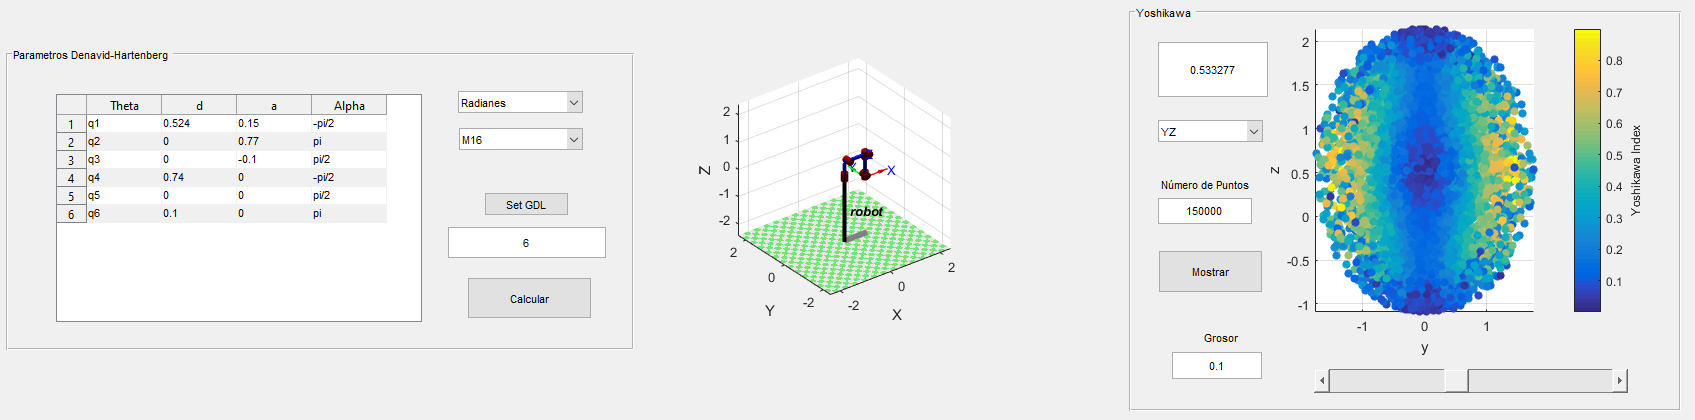
\includegraphics[width=1.0\linewidth]{images/Yoshi6.PNG}
		\caption{Visualización de índices de manipulabilidad de Yoshikawa para un robot de 6 GDL.}
		\label{Yoshi_6GDL}
	\end{figure}
	\FloatBarrier
	
	\subsection{Jacobiana}
	
	La \textbf{Jacobiana} establece la relación entre las velocidades de las articulaciones, con las velocidades del extremo del robot. Es utilizado por el sistema de control del robot para establecer qué velocidades debe imprimir a cada articulación para conseguir que el extremo desarrolle una trayectoria temporal concreta. También permite relacionar los pares de los actuadores con los que aparecen en el extremo del robot.\\
	
	\[
	\begin{bmatrix}
	\dot{x}\\
	\dot{y}\\
	\dot{z}\\
	\dot{\phi}\\
	\dot{\theta}\\
	\dot{\psi}
	\end{bmatrix}
	=
	\begin{bmatrix}
	\cdotp & \cdots & \cdotp\\
	\cdotp & \cdots & \cdotp\\
	\cdotp & \cdots & \cdotp\\
	\cdotp & \cdots & \cdotp\\
	\cdotp & \cdots & \cdotp\\
	\cdotp & \cdots & \cdotp
	\end{bmatrix}
	\begin{bmatrix}
	\dot{q}_1\\
	\dot{q}_2\\
	\dot{q}_3\\
	\vdots\\
	\dot{q}_n
	\end{bmatrix}
	\]
	
	La matriz Jacobiana se ha calculado en la función \textit{Jacobian(robot, qs, handles)}, en esta función se emplea el método:
	
	\begin{lstlisting}
	Jacob = robot.jacob0(qs);   
	\end{lstlisting}
	%
	Este método permite calcular la Jacobiana del robot con respecto al origen para las coordenadas articulares dadas.\\
	
	La Jacobiana puede descomponerse de la siguiente manera:
	
	\begin{myalign}
		\begin{split}
			v &= \vec{J}_{v1}\cdot \dot{q}_1 + \vec{J}_{v2}\cdot \dot{q}_2 + \ldots\\
	   \omega &= \vec{J}_{\omega1}\cdot \dot{q}_1 + \vec{J}_{\omega2}\cdot \dot{q}_2 + \ldots
		\end{split}
	\end{myalign}
	%
	Con esto podemos representar los vectores de la Jacobiana en dos \textit{plots} distintos, uno para la representación de la dirección del vector velocidad lineal del extremo y el otro para el angular. Un ejemplo para un robot de \textbf{3GDL} es el de la Figura \ref{Jacob_6GDL} para los siguientes valores de las articulaciones:
	
	\begin{myalign}
		\begin{split}
			q1 &= 45\\
			q2 &= 90\\
			q3 &= -90\\
			q4 &= 30\\
			q5 &= 25\\
			q6 &= 0
		\end{split}
	\end{myalign}	
	
	
	\begin{figure}[h!]
		\centering
		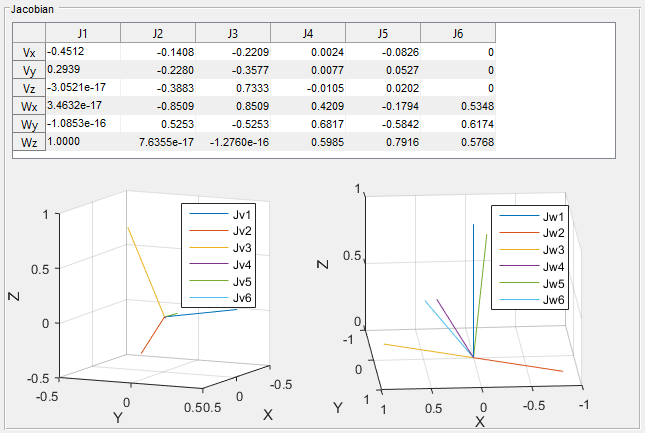
\includegraphics[width=0.8\linewidth]{images/Jacob6.PNG}
		\caption{Visualización la Jacobiana para un robot de 6 GDL.}
		\label{Jacob_6GDL}
	\end{figure}
	\FloatBarrier
	
	\section{Videos de Demostración} \label{Videos}
	
	He realizado tres vídeos de demostración del programa desarrollado para el presente trabajo. Los vídeos se encuentran en la siguiente carpeta de Dropbox, \href{https://www.dropbox.com/sh/8dfv6x28720glma/AAA1C-CvhHF4VmOJYF_xqjj6a?dl=0}{Carpeta de Dropbox con los tres vídeos.}
	
	\begin{description}
	\item[GDL3] Este vídeo contiene subtítulos en el que voy narrando todo el proceso. Presenta un robot de 3 grados de libertad precargado.
	\item[GDL6] Este vídeo no contiene subtítulos, ya que realizo las mismas actividades que en GDL3. Presenta un robot de 6 grados de libertad precargado.
	\item[Ejercicio4.2] Este vídeo, sin subtítulos tampoco, presenta el robot del Ejercicio 4.2 del libro de Fundamentos de Robótica\cite{Robotica}. Se van realizando algunos ejercicios del ejercicio, por ejemplo, sacar las matrices de transformación homogénea para ciertas coordenadas articuladas dadas.
	\end{description}
	
	\section{Pruebas de la Parte 2}
	
	Se han ido realizando distintas pruebas a lo largo del desarrollo de la \textbf{Parte 2}, la demostración de que el programa funciona están en los vídeos de la sección \ref{Videos}. Se dejará constancia en este documento de la realización de test en distintos robots en formato imagen.
		
	\begin{figure}[h!]
		\centering
		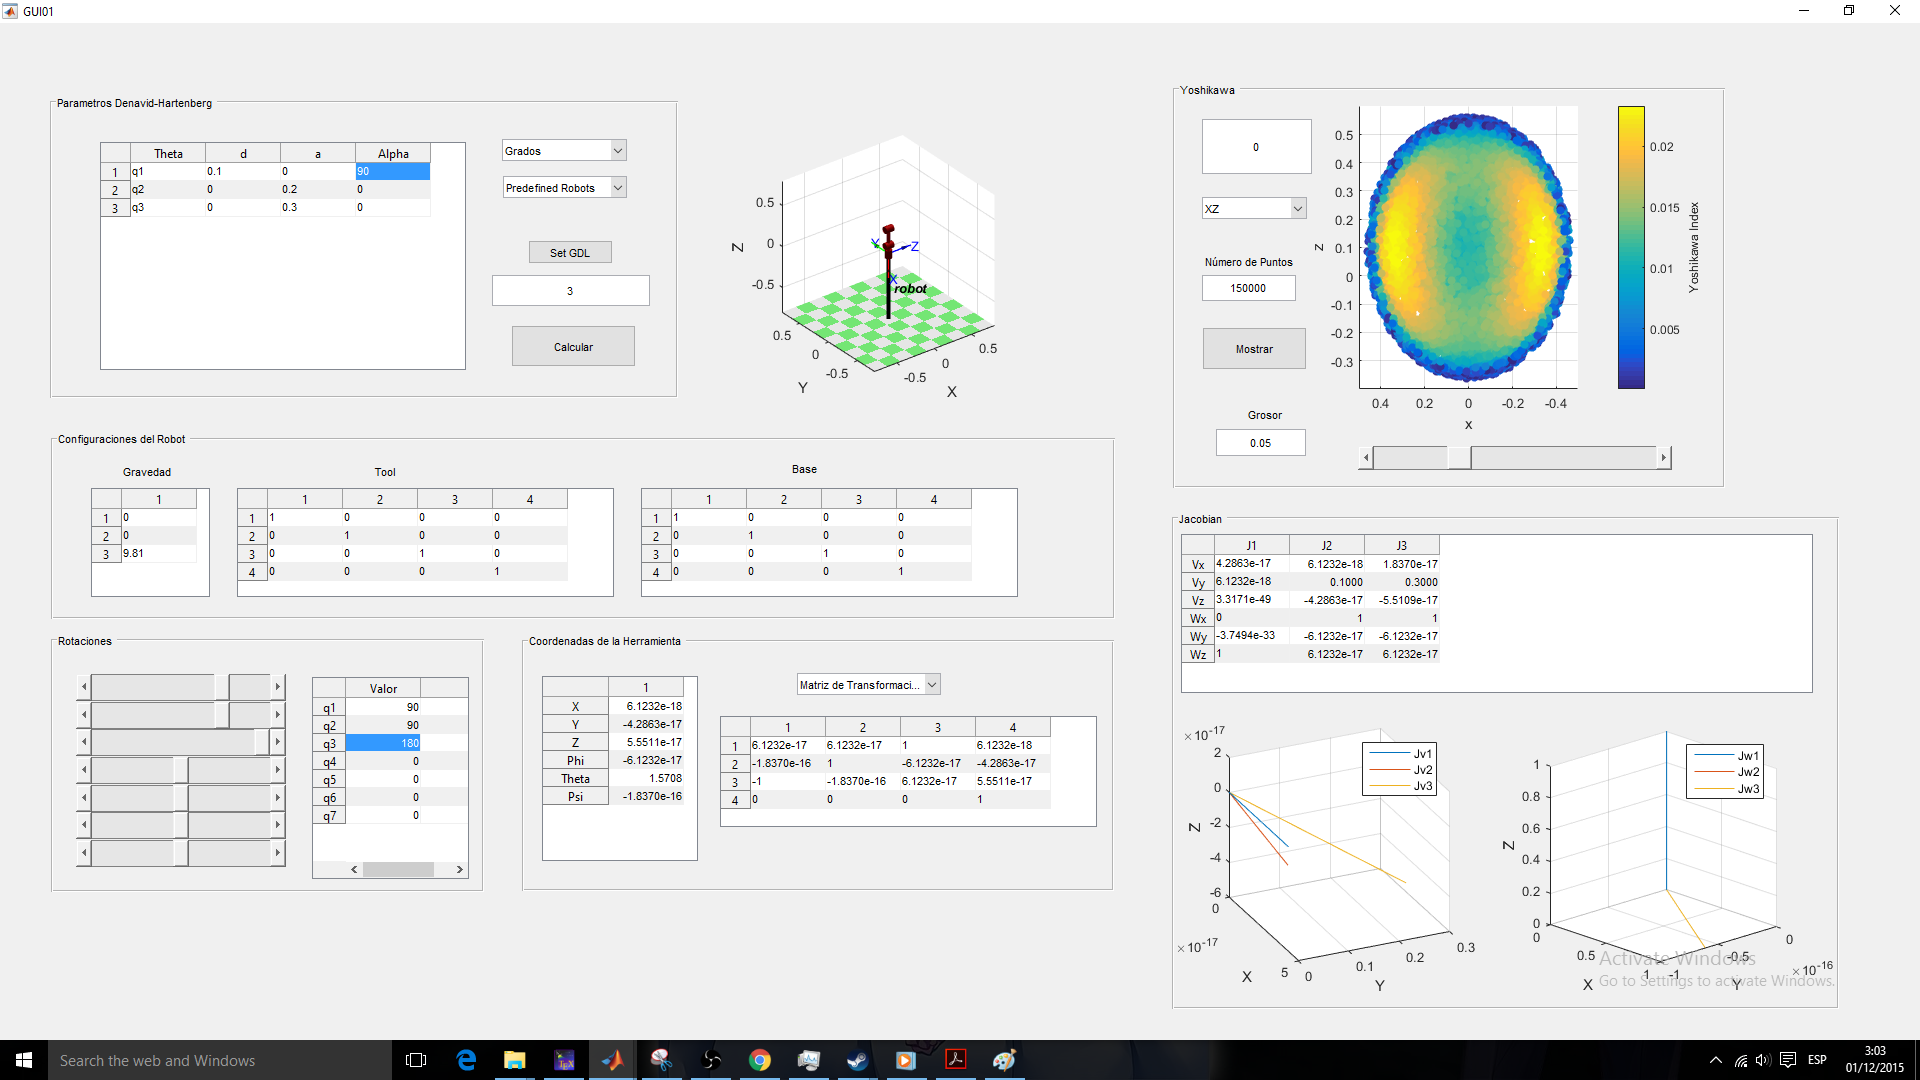
\includegraphics[width=1.0\linewidth]{images/Ejercicio42.PNG}
		\caption{Robot de 3 GDL del ejercicio 4.2, el cuál aparece en un vídeo.}
		\label{Ejercicio42}
	\end{figure}
	\FloatBarrier
	
	\begin{figure}[h!]
		\centering
		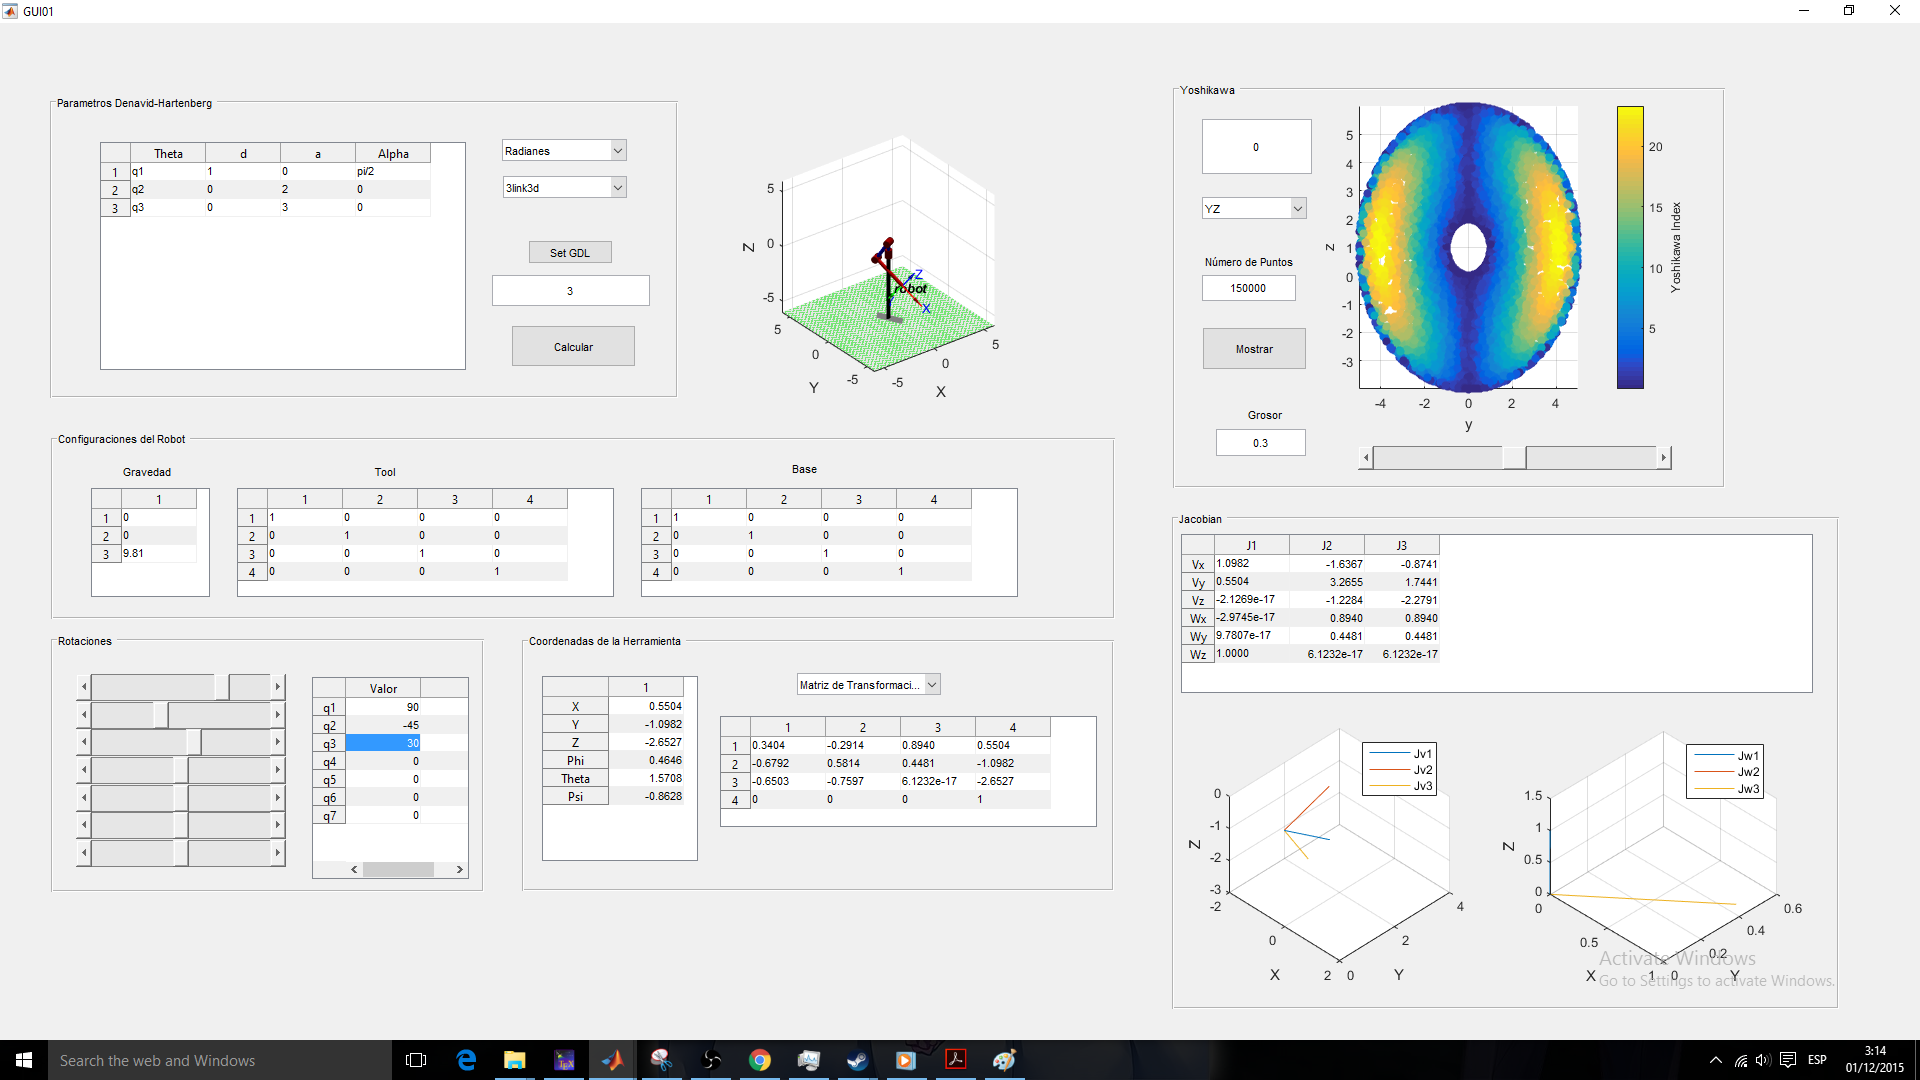
\includegraphics[width=1.0\linewidth]{images/3link3d.PNG}
		\caption{Robot de 3 GDL, \textit{3link3D} precargado en la toolbox.}
		\label{3link3D}
	\end{figure}
	\FloatBarrier
	
	\begin{figure}[h!]
		\centering
		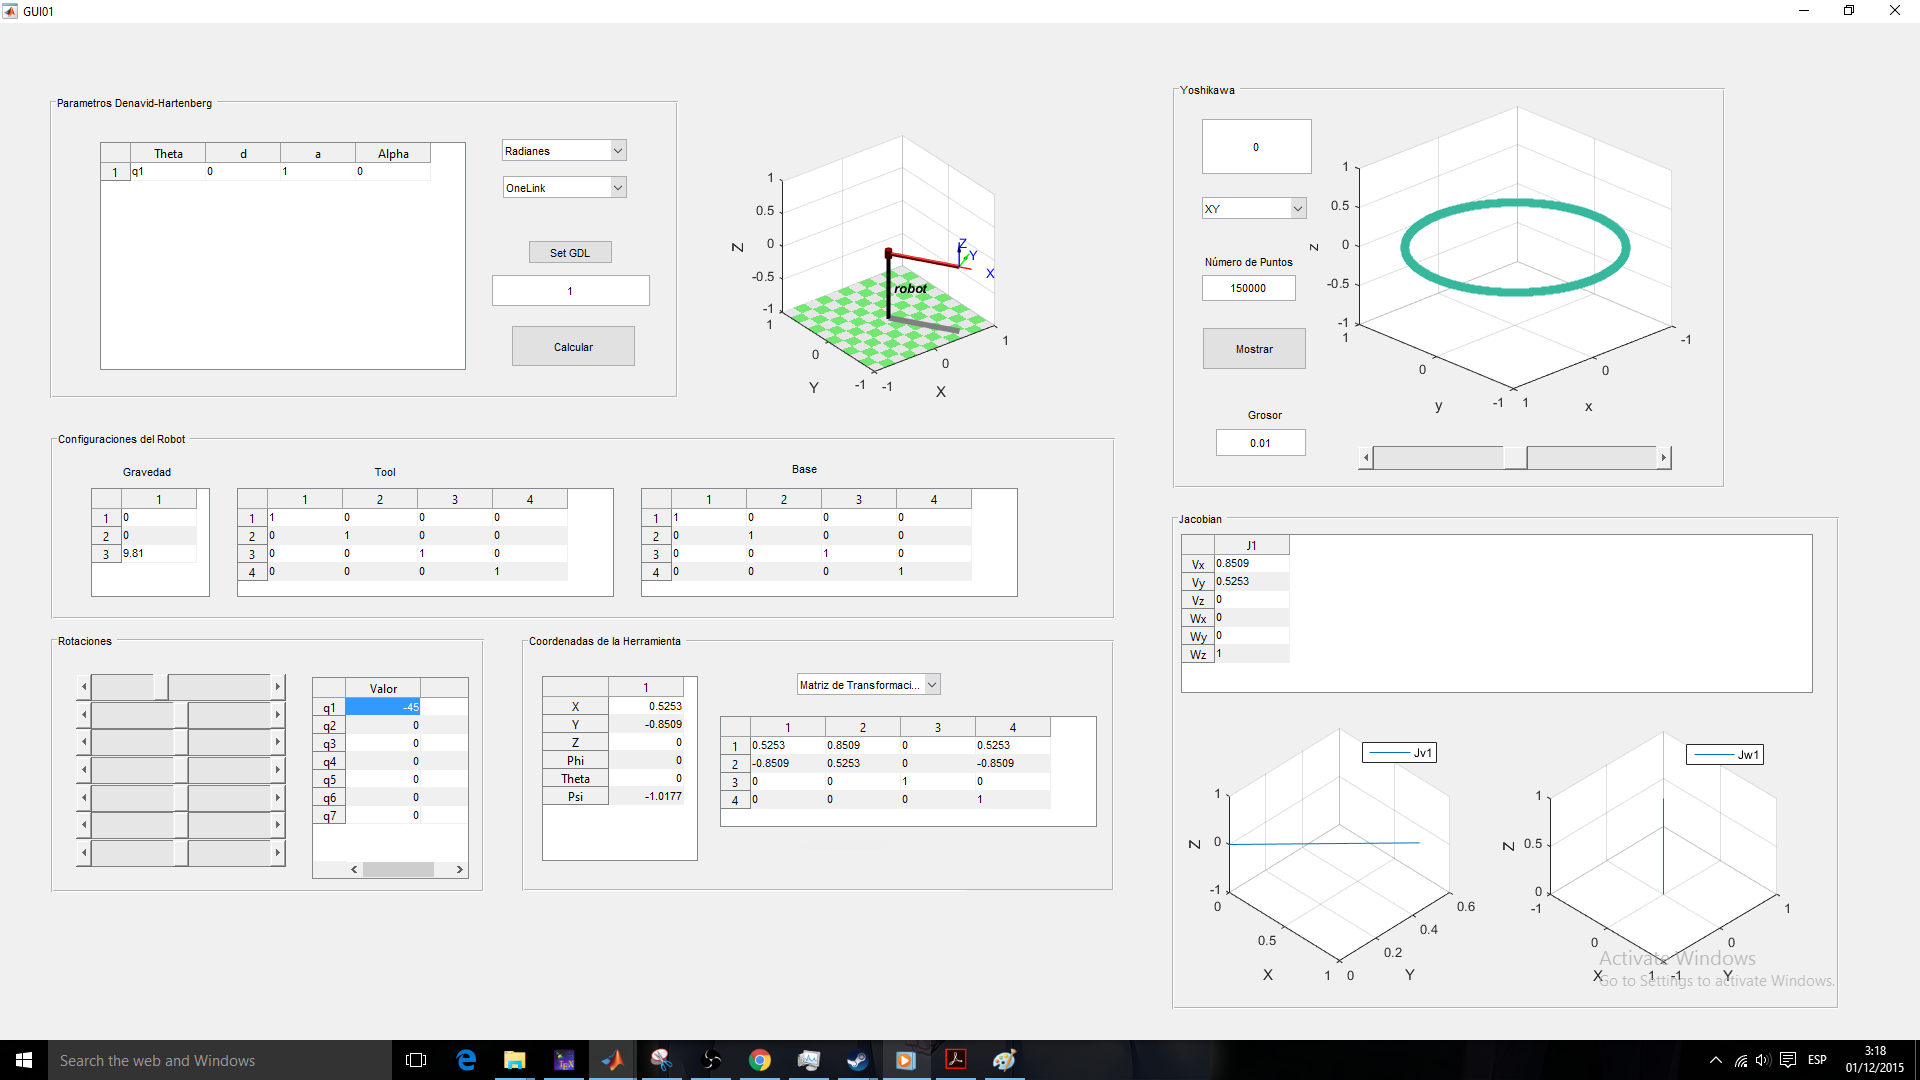
\includegraphics[width=1.0\linewidth]{images/OneLink.PNG}
		\caption{Robot de 1 GDL. Se observa en Yoshikawa que al tener nula manipulabilidad no se representan colores ya que es todo nulo. Además sale un círculo, ya que es el único movimiento que realiza.}
		\label{OneLink}
	\end{figure}
	\FloatBarrier
	
	\begin{figure}[h!]
		\centering
		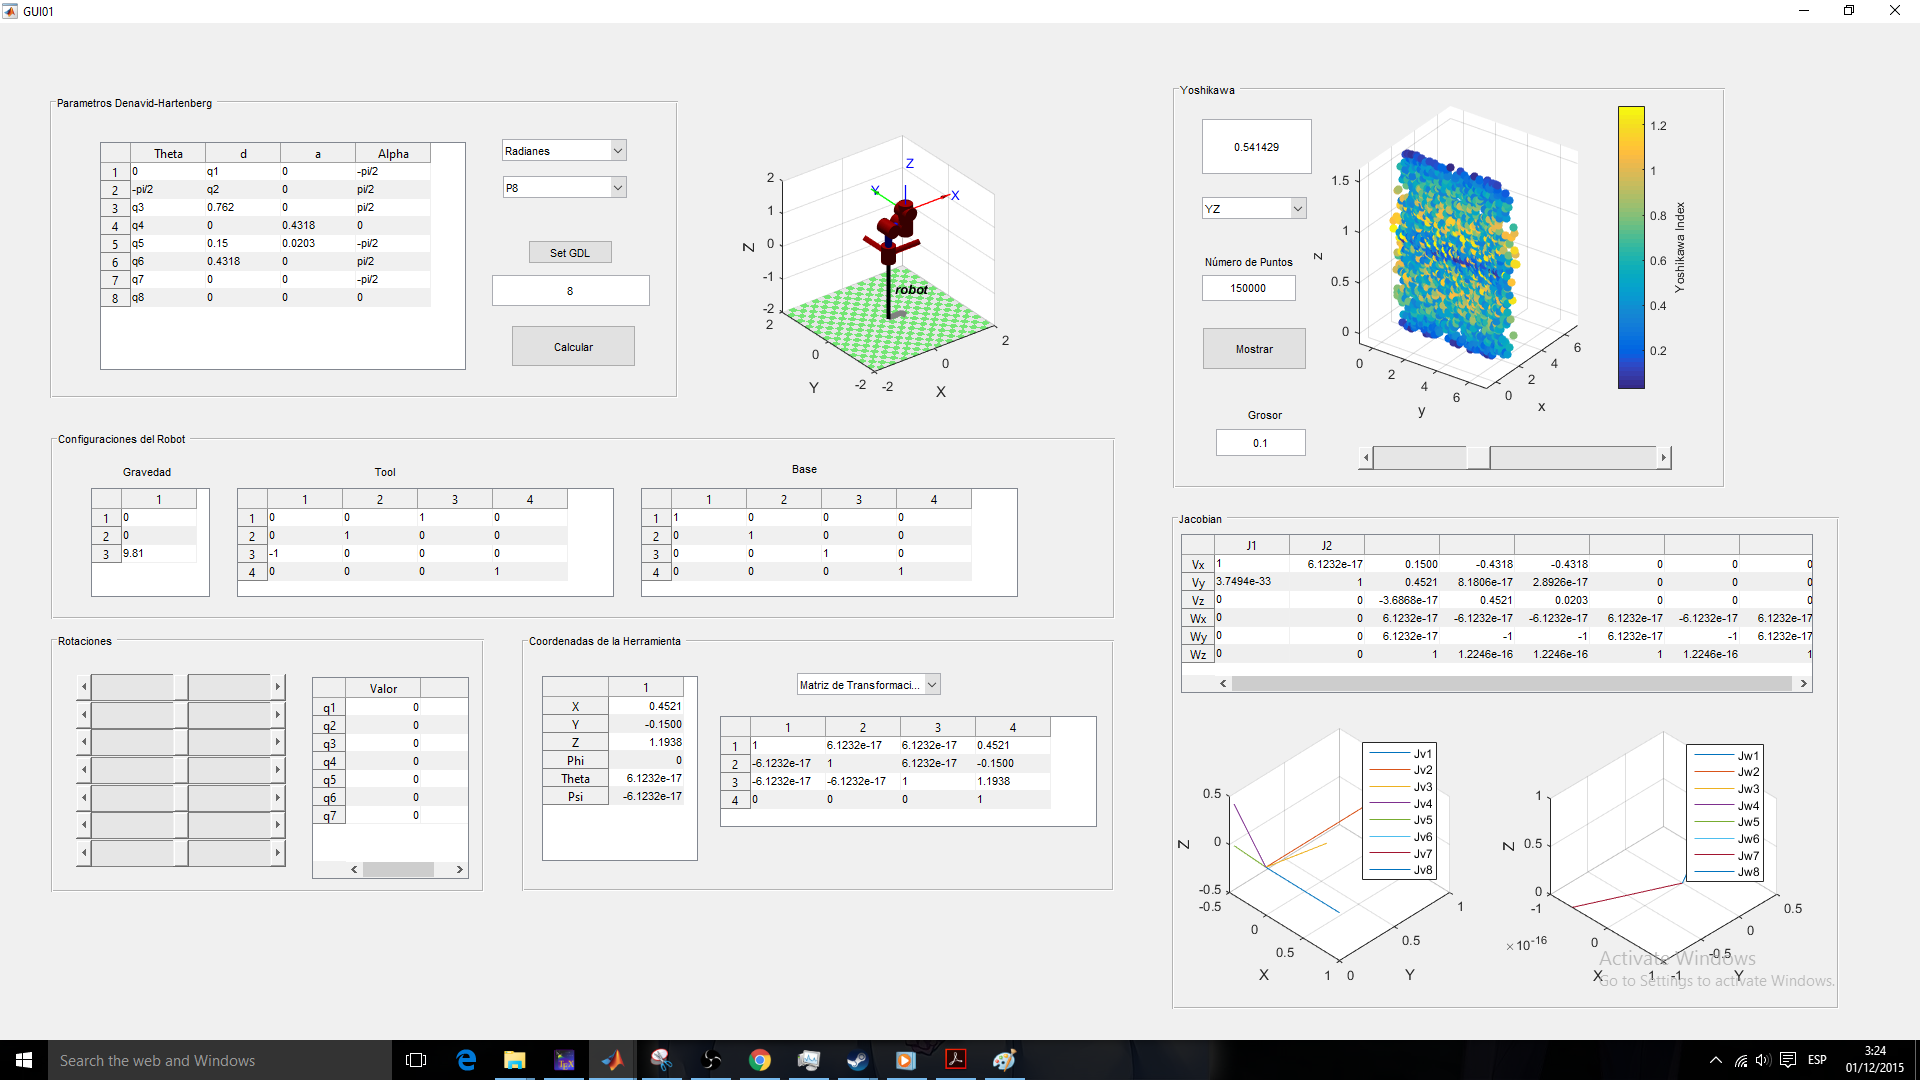
\includegraphics[width=1.0\linewidth]{images/P8.PNG}
		\caption{Robot de 8 GDL. Es el robot \textit{P8} de la toolbox.}
		\label{P8}
	\end{figure}
	\FloatBarrier

	\begin{figure}[h!]
		\centering
		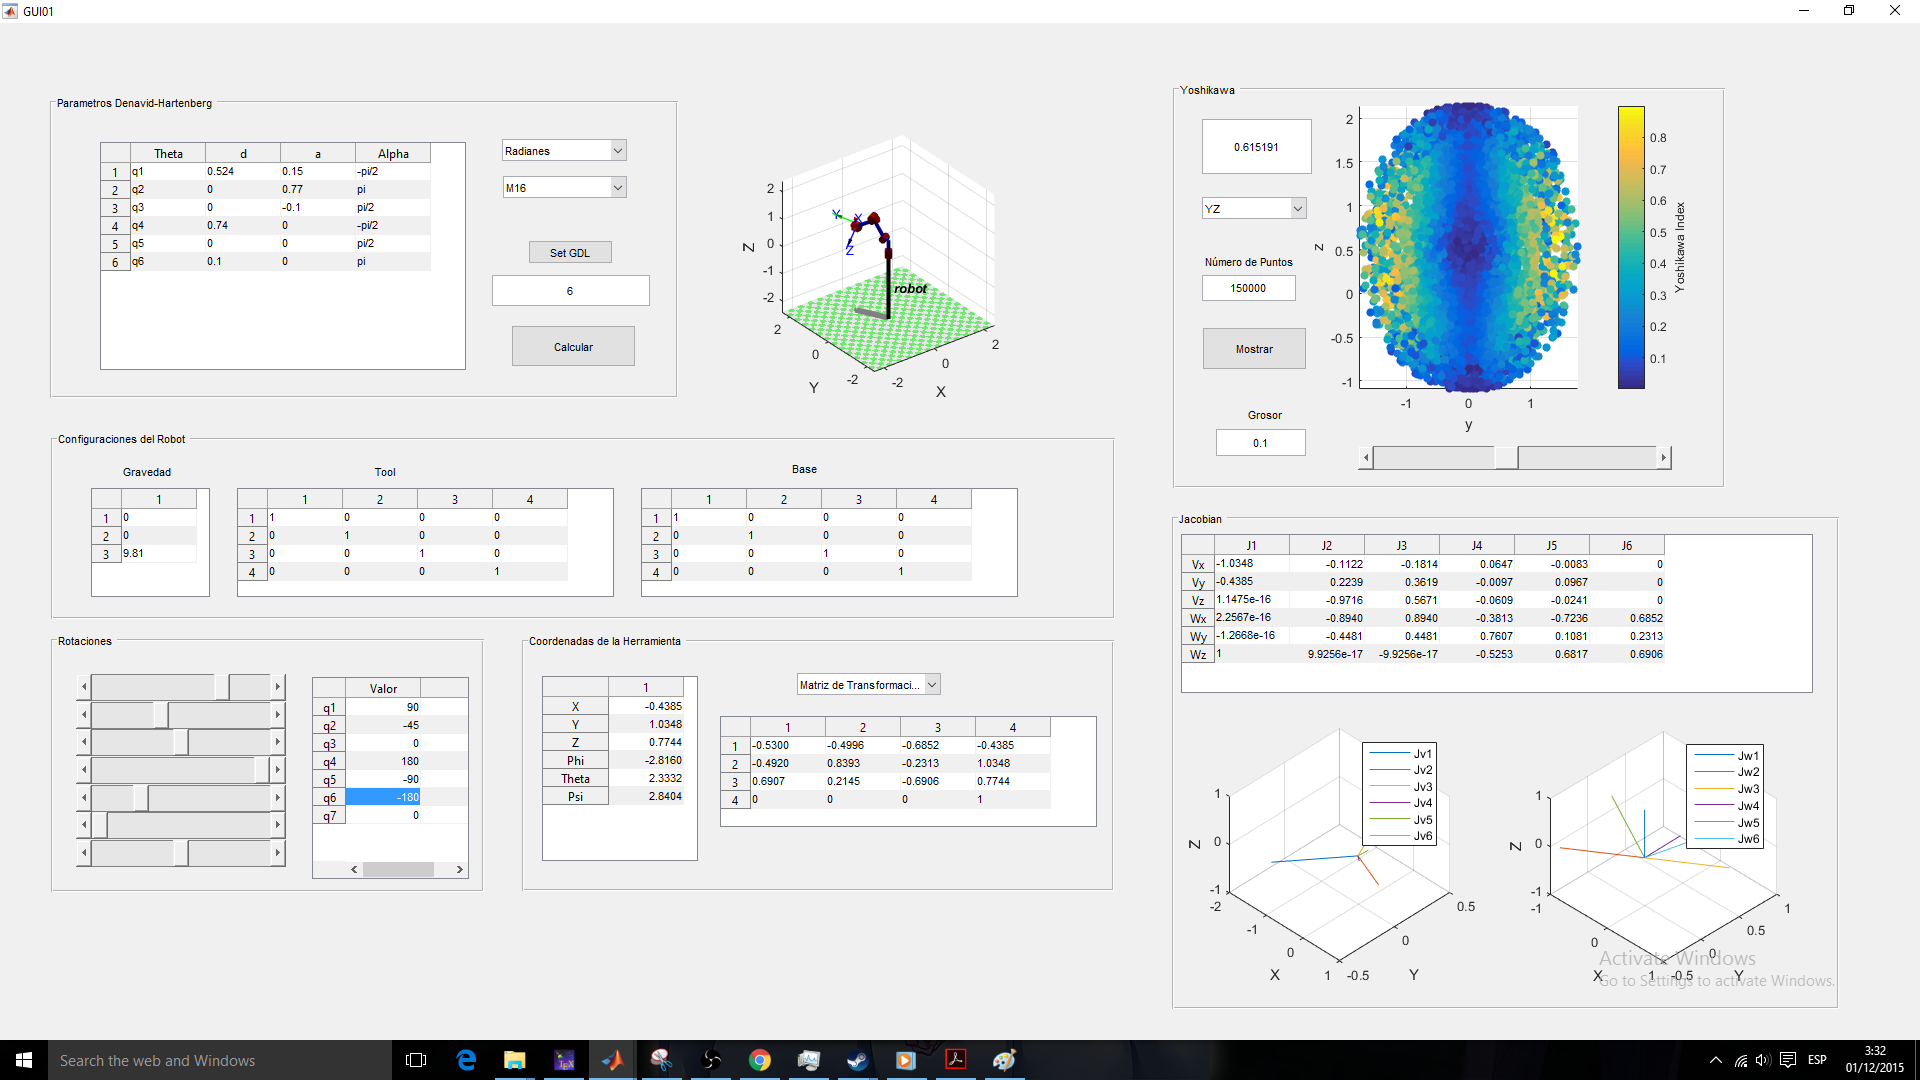
\includegraphics[width=1.0\linewidth]{images/M16.PNG}
		\caption{Robot de 6 GDL. Es el robot \textit{M16} de la toolbox.}
		\label{M16}
	\end{figure}
	\FloatBarrier

	\section{Mejoras a Futuro}
	
	A lo largo de la escritura del código me han surgido errores o problemas que por falta de tiempo o quedar fuera del alcance de este trabajo no he llegado a hacer.\\
	
	Un problema es que al hacer \textit{plot} del robot con la toolbox ancla la GUI en la parte superior de la pantalla impidiendo mover esta por la pantalla. Esto no he podido solucionarlo al tratarse de un bug del código de la toolbox y no he tenido tiempo de depurarlo. Se soluciona manualmente redimensionando la ventana en Windows, en Linux o en OSX no sé si dará fallo y si da esta solución no sé si también funcionará.\\
	
	Otro problema que surge con el mismo \textit{plot} es que si tienes coordenadas prismáticas y haces \textit{plot} surge un error, que se soluciona al darle los límites del volumen del \textit{workspace}, de momento lo mantengo fijo en [-2 2 -2 2 -2 2], pero de cara al siguiente trabajo he pensado modificarlo dinámicamente en función de la posición de la herramienta u otros parámetros, el problema de emplear la posición de la herramienta es que no tiene porqué ser la parte más alejada del robot. Otra solución es la suma de ciertos parámetros prismáticos de DH y emplearlos para delimitar el \textit{workplace}.\\
	
	Otra opción que me gustaría implementar es que al cargar un robot predefinido se puedan establecer con parámetros rotativos de DH en grados sexagesimales.\\
	
	Pero la principal tarea extra sería la generación dinámica de los \textit{sliders} de rotaciones en función de los gdl establecidos. Así se podrá controlar todas las rotaciones de un robot de más de 7 grados de libertad, que es el máximo que se puede actualmente.\\

	También seguiría introduciendo nuevos robots predefinidos e incluso poder incluir múltiples robots a la vez en los cálculos, por ejemplo el robot \textit{Baxter} está formado por dos robots (brazos) independientes, el izquierdo y el derecho. Sería muy interesante poder incluir esta opción.\\
	
	\bibliographystyle{acm} % estilo de la bibliografía.
	\bibliography{yyyy} 
	
	\begin{thebibliography}{X}
		
		\bibitem{ToolBoxRobotic} \textsc{Peter Corke} \textit{Robotics, Vision and Control. Fundamental Algorithms in Matlab}, Springer Tracs in Advanced Robotics.
		
		\bibitem{Robotica} \textsc{Antonio Barrientos, Luis Felipe Peñín, Carlos Balaguer} y \textsc{Rafael Aracil} \textit{Fundamentos de Robótica}, Segunda Edición, McGrawHill, 2010.
		
	\end{thebibliography}
	
\end{document}